
\documentclass[letterpaper, 11pt]{report}
\usepackage[utf8]{inputenc}
\usepackage{titlesec}
\usepackage{fullpage} % changes the margin
\usepackage{graphicx} %package to manage images
\graphicspath{ {./images/} }

\begin{document}
\begin{titlepage}
\vspace*{0.7in}
\begin{center}
\begin{figure}[htb]
\begin{center}

\includegraphics[width=8cm]{univ_logo}
\end{center}
\end{figure}
\vspace*{0.3in}
\begin{Large}
\textbf{SOEN 6011 : SOFTWARE ENGINEERING PROCESSES} \\
\end{Large}
\vspace*{0.1in}
\begin{Large}
\textbf{SUMMER 2021} \\
\end{Large}
\vspace*{0.9in}
\begin{Large}
\textbf{SUPER CALCULATOR} \\
\end{Large}
\vspace*{0.9in}
\begin{Large} 


\textbf{PROBLEM - 5} \\
 Source Code Review\\
\end{Large}
\vspace*{0.625in}
\rule{80mm}{0.1mm}\\
\vspace*{0.1in}
\begin{large}
Authors \\
\vspace*{0.1in}
Rokeya Begum Keya\\
\vspace*{0.1in}
Kyle Taylor Lange\\
\vspace*{0.1in}
Sijie Min\\
\vspace*{0.1in}
Manimaran Palani\\ 
\vspace*{0.3in}
\date{\normalsize\today} 
\end{large}
\end{center}
\begin{center}
https://www.overleaf.com/project/610304de4e6b8d24f7c781b6\end{center}
\end{titlepage}
\tableofcontents
\newpage
\section*{\centering{PROBLEM 5 - F2: $tan(x)$}}
\normalsize {SOEN 6011 - Summer 2021} \hfill \textbf{Rokeya Begum Keya} \\
\textbf{ Software Engineering Processes}  \hfill \textbf{40183615} \\
\hfill Repository address : https://github.com/Dakatsu/SOEN6011Calculator
\\
\addcontentsline{toc}{section}{a) Source code Review of F3 }
\section*{Source code Review of F3}
The report of source code review for Hyperbolic Sine, $sinh(x)$ function: Developed by Kyle Taylor Lange.
\section*{Manual Code Review}
\subsection*{Naming Conventions }
The class name, variables, constant variables and methods are named according to the Java Naming Conventions.Java.
\subsection*{JavaDoc Comments}
\textbf{SinhLibrariesTest.java} - It would be better to quickly understand the Unit test methods if Javadoc comments are on the test cases.\\\
\begin{center}
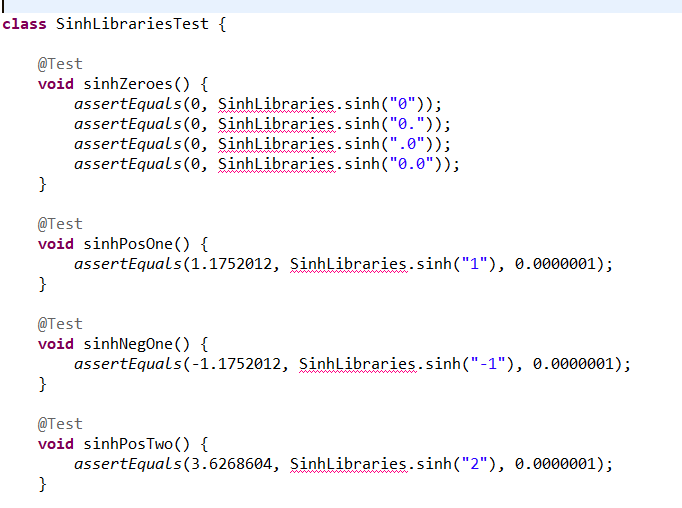
\includegraphics[width= 12cm]{F3_Code_Review_UTC}
\end{center}
\begin{center}
Figure 1: JavaDoc comments in test methods is missing 
\end{center}
\newpage
\section*{Automatic Code Review}
Automatic source code review is done by  \textbf{CheckStyle}\cite{CheckStyle} plug-in in eclipse IDE. I used google-check-global to review the code. I underline four errors which, are needed to be fixed, is given below in the figure 2.  \\\\
\begin{center}
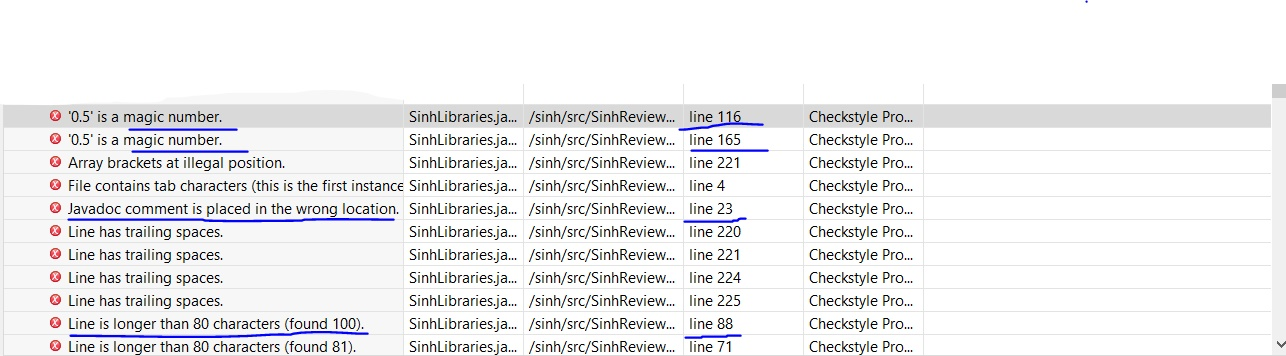
\includegraphics[width= 14cm]{F3_Code_Review_Checkstyle}
\end{center}
\begin{center}
Figure 2: Errors found by Checkstyle \end{center}
\pagebreak

\section*{\centering{PROBLEM 5 - F3: Hyperbolic Sine, $sinh(x)$}}
\normalsize {SOEN 6011 - Summer 2021} \hfill \textbf{Kyle Taylor Lange} \\
\textbf{ Software Engineering Processes}  \hfill \textbf{27627696} \\
\hfill Repository address : https://github.com/Dakatsu/SOEN6011Calculator
\\
\addcontentsline{toc}{section}{b) Source code Review of F5 }
\section*{Source code Review of F5}

I used Google's code review guidelines \cite{googleCodeReview} to review Sijie's code for function F5. The $calculate()$ function is the main function in F5.java, which returns the value of $ab^x$. This function simply calls a separate function for $b^x$ and multiplies that result by a, which makes sense from a reuse standpoint. \\\\
One confusing aspect was that there are two functions named $power()$, and the comment did not make it apparent that one takes a double exponent while the other takes an integer. The functions could be renamed to make this clearer. e.g. $powerInt$ and $powerDouble$, or the main body of the comments could be altered to make this clearer to those unfamiliar with how exponents relate to logarithms. \\\\
In any case, the double version of $power$ appears syntactically correct. It returns 1 or 0 if the exponent or base are 0, respectively, and then it relies on separating the integer from the decimal portion of the base similarly and calculates the base raised to the integral power times Euler's number raised to a power with a function called $ex$. \\\\
The $ex$ function has a confusing name, as I presumed it was short for exponent. Its Javadoc comment does clear this up, but perhaps renaming the function to something more detailed, e.g. $eToX$ or $naturalExp$ would make it clearer to casual users of this library. \\\\
The names of the functions and variables all conform to basic style guidelines, with constant values written in all caps and method/variable names written in camelCase. The main exception are the multiple variable names that are written as just a single letter, e.g. $a$ or $x$. This was difficult to read since I had to constantly refer to the Javadoc comments to remember which variable represented what. There are very few comments in the body of the functions themselves. This may not be necessary for some of the shorter functions, but certain functions took a bit of effort to understand what was occurring. \\\\
These functions were unfortunately not integrated into the main calculator program, so I was unable to review how the code worked in practice. Nevertheless, it passes all unit tests.

\begin{thebibliography}{}
\bibitem{googleCodeReview}
How to do a code review, \textit{Google}
\\https://google.github.io/eng-practices/review/reviewer/
\end{thebibliography}

\pagebreak

\section*{\centering{PROBLEM 5 - F5}}
\normalsize {SOEN 6011 - Summer 2021} \hfill \textbf{Sijie Min} \\
\textbf{ Software Engineering Processes}  \hfill \textbf{40152234} \\
\hfill Repository address : https://github.com/Dakatsu/SOEN6011Calculator
\\

\section*{Source code Review of F7}
Here is the source code review of a  Transcendental function (F7) - $x^y$ : Developed by Manimaran Palani.
\section*{Manual Code Review}
\subsection*{Source File Naming}
The code conforms to the google code style, and the method names and variable names in the code conform to the standard of camel case nomenclature
\subsection*{JavaDoc Comments}
Javadoc is added to classes and methods to facilitate the formation of highly readable documents with the project and to facilitate code understanding. But there is a lack of comments inside the function, you can add comments appropriately to help understand the code\\\\
\begin{figure}[htp]
    \centering
    \includegraphics[width=16cm]{F5p51}
    \caption{review F7.1}
    \label{fig:galaxy}
\end{figure}
\begin{figure}[htp]
    \centering
    \includegraphics[width=16cm]{F5p52}
    \caption{review f7.2}
    \label{fig:galaxy}
\end{figure}
\section*{Automatic Code Review Review of F7}
\\Use CheckStyle for automatic code review, the following figure PowerFunction.java and CheckStyle violations chart of PowerFunctionTest.java.
\begin{figure}[htp]
    \centering
    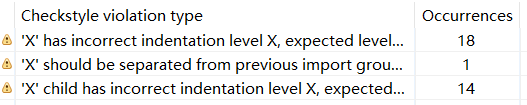
\includegraphics[width=16cm]{SOEN_6011-Problem-5/f5111.png}
    \caption{review of f7}
\end{figure}
\\I checked the naming convention issues that are easy to ignore through CheckStyle, as shown in the  picture

\begin{figure}[htb]
    \centering
    \includegraphics[width=16cm]{F5222}
    \caption{check style of f7}
    \label{fig:galaxy}
\end{figure}

 \begin{thebibliography}{}
 
\bibitem{test1}
Mike Spivey. "The fuzz Manual" Manual and software copyright . J. M. Spivey 1988, 1992, 2000


\end{thebibliography}  
\newpage
\\
\\
\\
\\
\\
\\
\\
\\
\\
\\
\\
\\
\\
\\
\\
\\
\\
\\
\\

\section*{\centering{PROBLEM 5 - F7 : \(x^y\)}}
\normalsize {SOEN 6011 - Summer 2021} \hfill \textbf{Manimaran Palani} \\
\textbf{ Software Engineering Processes}  \hfill \textbf{40167543} \\
\hfill Repository address : https://github.com/Dakatsu/SOEN6011Calculator
\\
\addcontentsline{toc}{section}{d) Source code Review of F2 }
\section*{Source code Review of F2}
This sections presents the source code review of a  Transcendental function (F2) - $tan(x)$ : Developed by Rokeya Begum Keya.

\section*{Manual Code Review}
\subsection*{Source File Naming}
The class name and methods are named as per Java Naming Conventions.Java uses Camel-Case as a practice for writing names of methods, variables, classes, packages and constants.
\subsection*{JavaDoc Comments}
Javadoc is a tool which comes with JDK and it is used for generating Java code documentation in HTML format from Java source code, which requires documentation in a predefined format.\\\\
\textbf{TangentFunction.java} - Methods and variables declared in the class can have appropriate JavaDoc to have a better readability of the code.\\
\begin{figure}[htb]
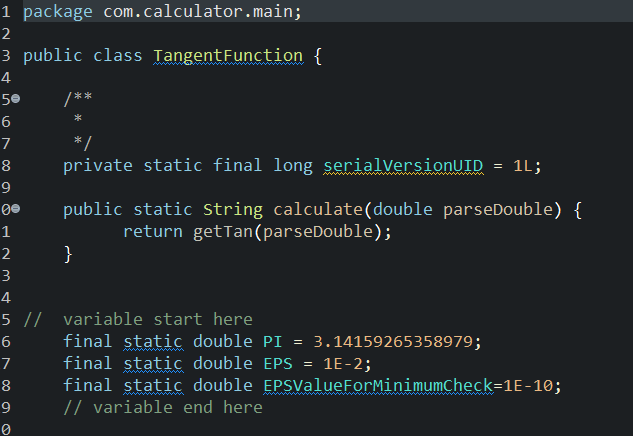
\includegraphics[width=0.5\textwidth]{F2_Code_Review_JavaDoc}
\centering
\caption{Missing JavaDoc comments in methods and variable declarations}
\end{figure}
\\\\\\
\textbf{TangentFunctionTest.java} - Unit test methods in the class can have Javdoc comments to quickly understand the purpose of the test cases.
\begin{figure}[htb]
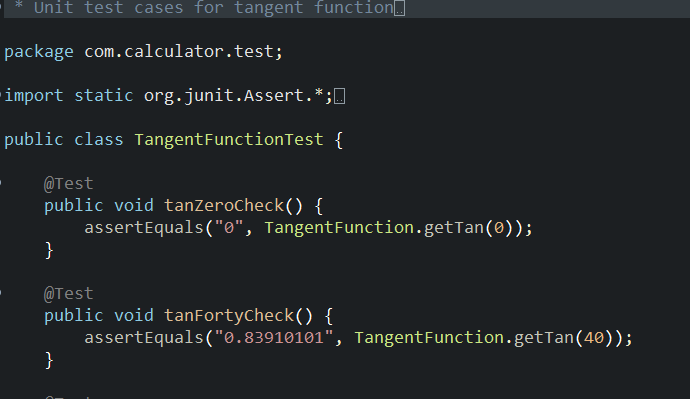
\includegraphics[width=0.6\textwidth]{F2_Code_Review_JavaDoc_TestCase}
\centering
\caption{Missing JavaDoc comments in test methods}
\end{figure}
\section*{Automatic Code Review}
Automatic source code review is done by  \textbf{CheckStyle}\cite{CheckStyle} plugin integrated with eclipse IDE which is available in the form of plugin.\\\\
Checkstyle inspects Java source code and pointing out items that deviate from a defined set of
coding paradigms.\\\\
\begin{figure}[htb]
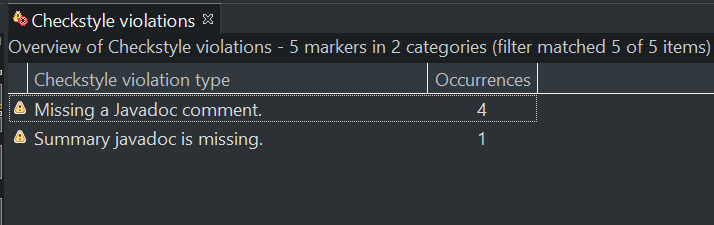
\includegraphics[width=0.7\textwidth]{F2_Code_Review_CheckStyle_Violation}
\centering
\caption{TangentFunction.java - CheckStyle Violation}
\end{figure}
\begin{figure}[htb]
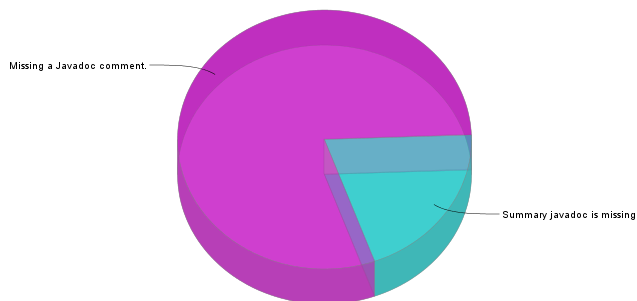
\includegraphics[width=0.6\textwidth]{F2_Code_Review_CheckStyle_Violation_Graph}
\centering
\caption{TangentFunction.java - CheckStyle Violation Graph}
\end{figure}
\begin{figure}[htb]
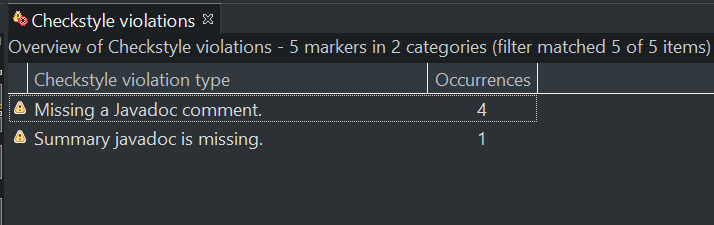
\includegraphics[width=0.7\textwidth]{F2_Code_Review_CheckStyle_Violation}
\centering
\caption{TangentFunctionTest.java - CheckStyle Violation }
\end{figure}
\begin{figure}[htb]
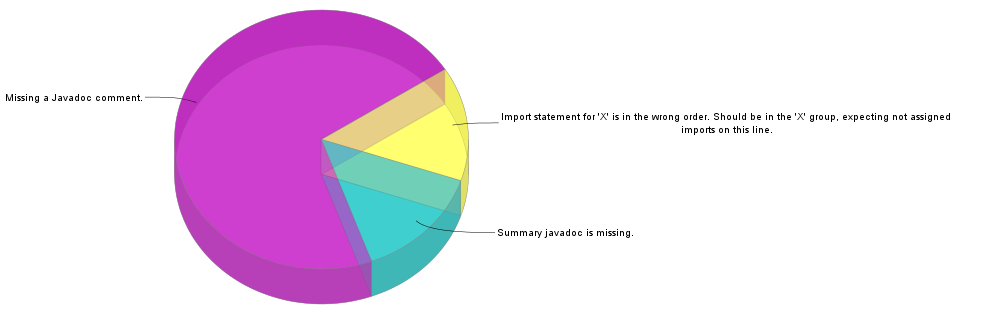
\includegraphics[width=0.6\textwidth]{F2_Code_Review_CheckStyle_Violation_Graph_TestCases}
\centering
\caption{TangentFunctionTest.java - CheckStyle Violation Graph}
\end{figure}

\begin{thebibliography}{}
\bibitem{CheckStyle} 
 CheckStyle. Eclipse Checkstyle Plugin. 2019.
\\\texttt{ https://checkstyle.org/eclipse-cs}
\end{thebibliography}
\end{document}
